\section{Introduction}\label{sec:introduction}
\subsection{Context}
	The suspension on a mountain bike plays a vital part in the rider's performance, comfort and overall enjoyment of the sport. With some suspension units costing upwards of \pounds1000 it is vital that they are setup to function correctly. The objective of this dissertation is to examine how image analysis can be used in the set-up of mountain bike suspension, and produce a prototype application that helps beginner and intermediate riders to carry out an initial set-up.
\subsection{Background}
	A survey carried out by the International Mountain Bike Association found that the average price had paid for a mountain bike was \euro2546 (\pounds2206) \citep{imbasurv}. Starting at approximately \pounds1000 \citep{giantstance}, enthusiast level mountain bikes can be purchased with suspension for both the front and rear wheels, known as \gls{fs} bikes whereas \gls{ht} bikes only have front suspension units; this difference can be seen in Figure \ref{fig:fsandht}. The price of higher specification mountain bikes can run to many thousands of pounds, but even entry level models are equipped with adjustable suspension units that need to be correctly configured to the rider's weight and the characteristics of the terrain.
	\begin{figure}[h!]
		\centering
		\begin{minipage}{0.45\textwidth}
			\centering
			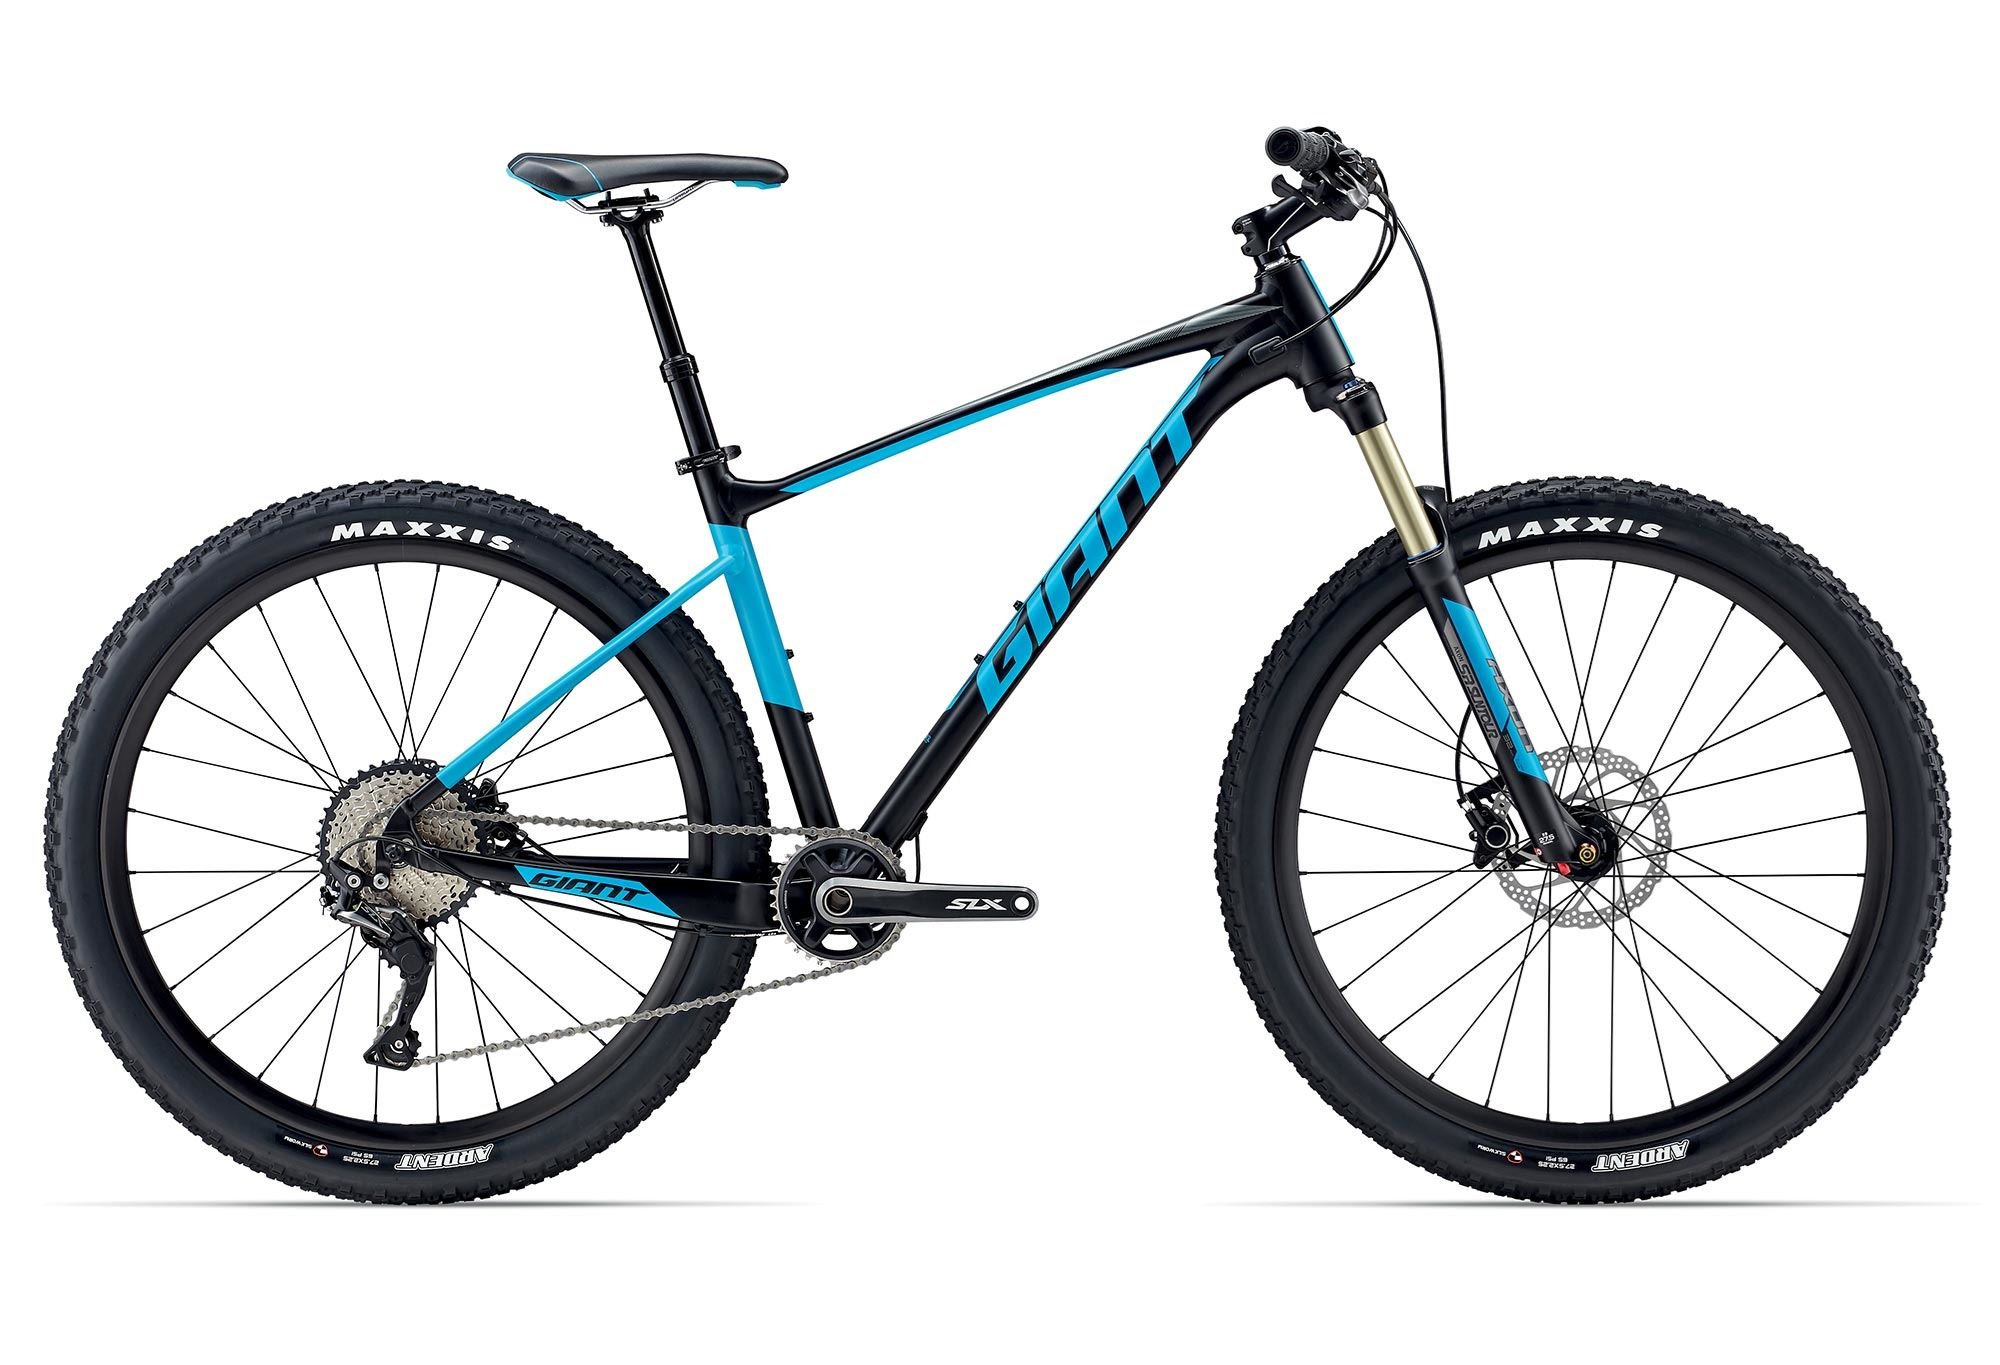
\includegraphics[width=7cm]{../images/2017_GIANT_FATHOM_1.jpg}
		\end{minipage}\hfill
		\begin{minipage}{0.45\textwidth}
			\centering
			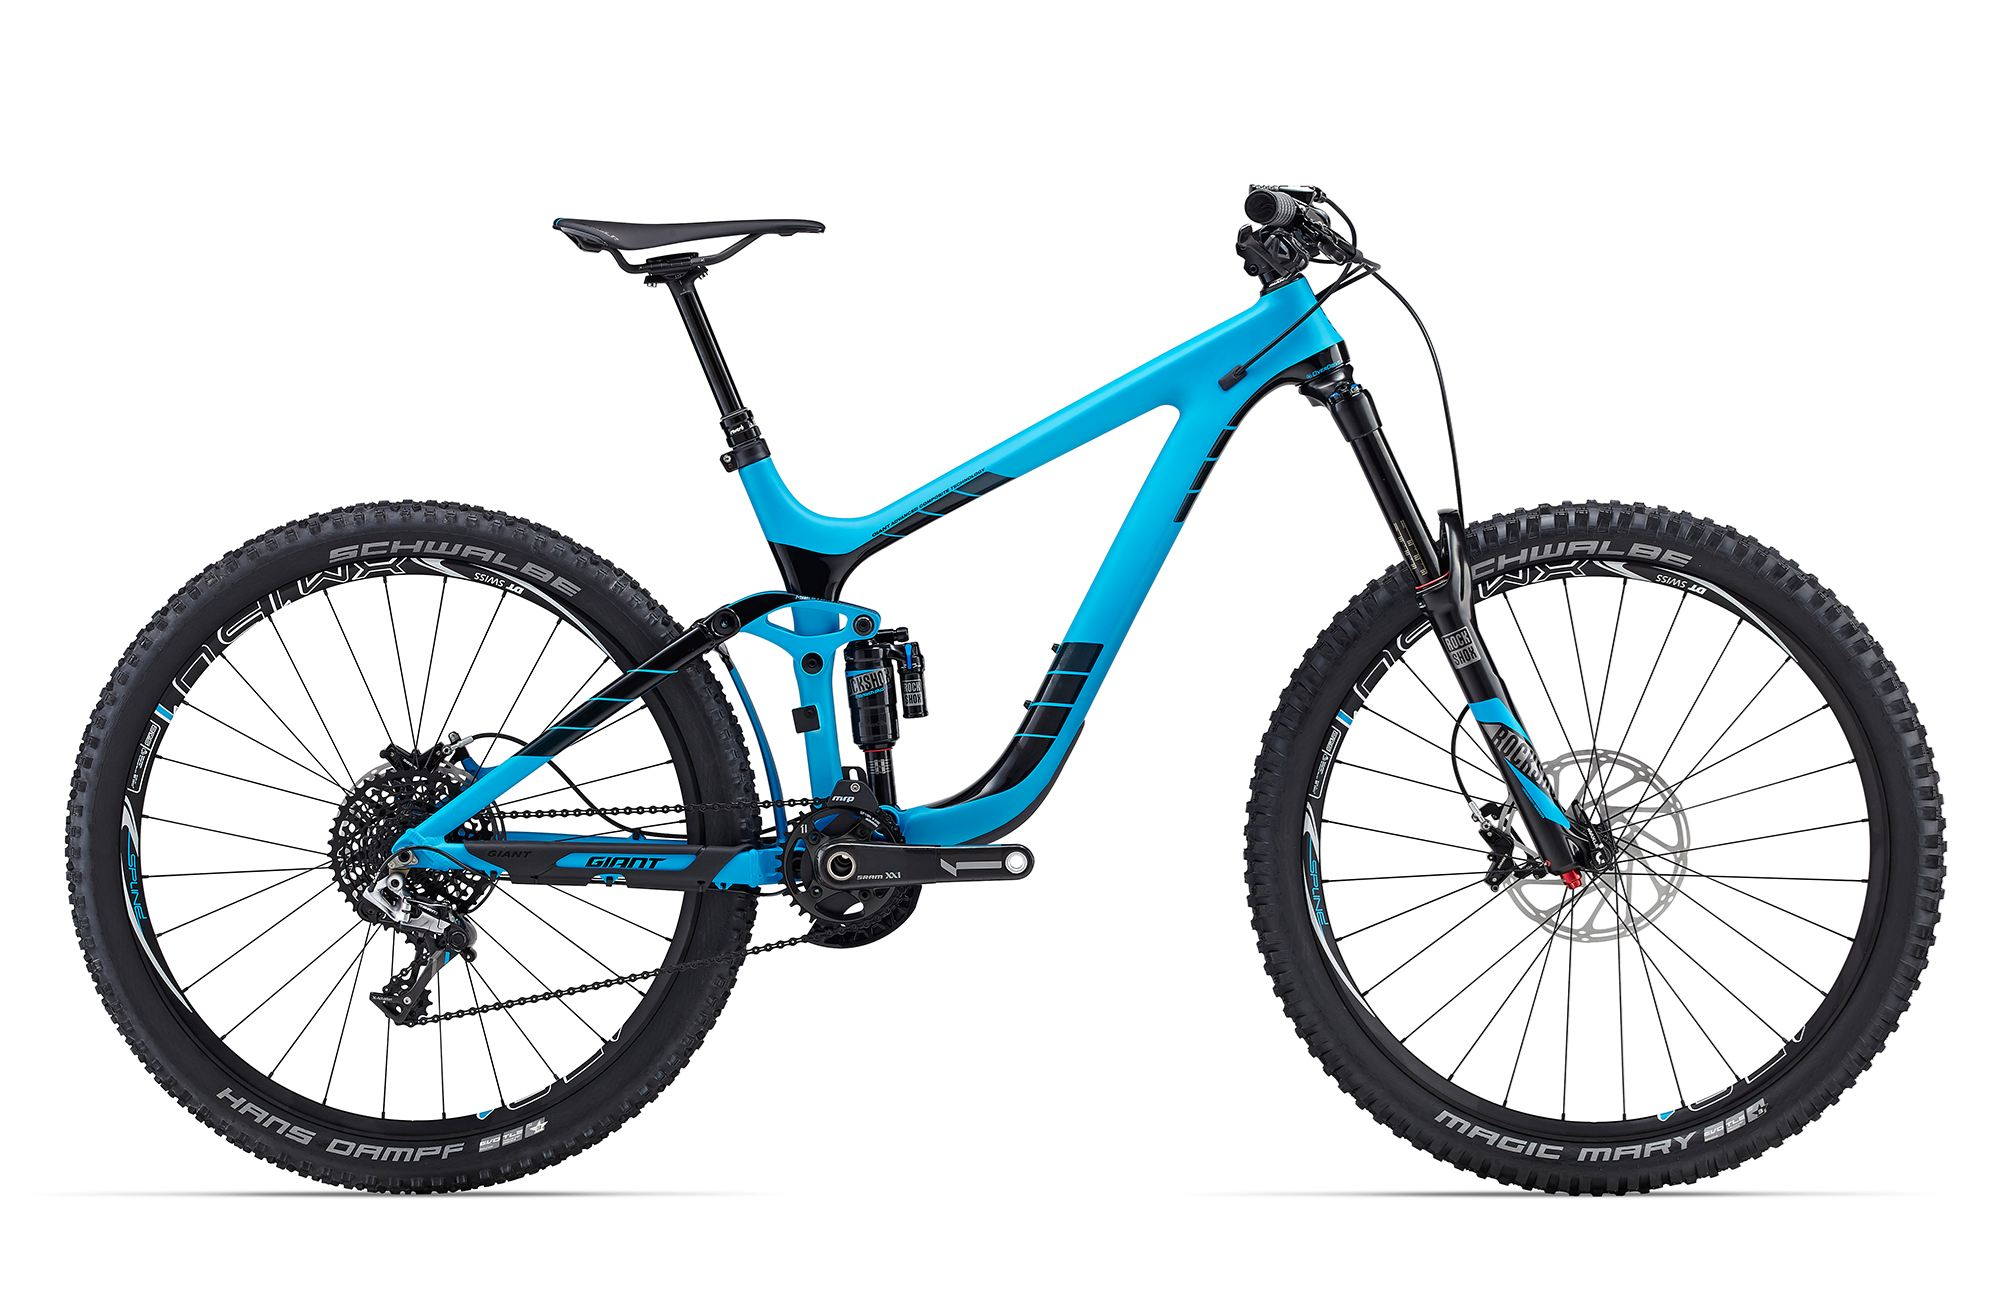
\includegraphics[width=7cm]{../images/2016_Giant_Reign_Advanced_275_0.jpg}
		\end{minipage}
		\caption{Hardtail and full suspension mountain bikes \citep{giantfathom,giantreign}}
		\label{fig:fsandht}
	\end{figure}
	\\
	It has been proven that using a FS bike as opposed to a HT gives the rider a measurable performance advantage \citep{fullsusperf}. However, if the suspension fork and/or rear shock have not been correctly configured it can be detrimental to the rider’s performance and potentially lead to injury. For example, if a \gls{shock} has too little \gls{rebounddamping} set and the rider goes off a jump, the excessive speed at which the	rear of the bike extends can create forwards rotation, causing the rider to go over the handlebars of the bike. However many enthusiasts lack the specialist knowledge required to optimize the set-up of their bike’s suspension units and as a consequence compromise their performance and riding experience.
	\\\\
	Additionally, an incorrect suspension setup can cause excessive wear and tear on the	bike’s frame and components. For instance, suspension which is set too soft will cause “bottoming out” where the unit reaches the end of its available range so that excess forces are transferred to the frame causing stress and potentially dramatic fracture that could result in injury. Conversely, suspension that is set too hard forces energy that would normally be absorbed to the wheels resulting in denting and warping of the rims.
	\\\\
	Many bicycle retailers will configure the suspension of a newly purchased mountain bike for the customer at the time of collection. Most of the time this will be enough to avoid incident but as the customer is unlikely to be wearing weighty protection equipment and accessories such as helmet, body armour and hydration pack, this initial setup is rarely accurate. Furthermore, with some manufacturers choosing direct sales over
	local retailers \citep{roseonline,ytonline}, even this rudimentary setup can be omitted altogether.
	\\\\
	Since the birth of the modern smartphone in 2007, brought about by the first generation Apple® iPhone® and introduction of the Android™ mobile operating system, the use of mobile computing in everyday life has grown rapidly. Google™ stated that there were approximately 1.4 billion active Android users worldwide in 2015 \citep{androidusers}.
	\\\\
	The introduction of activity tracking devices and mobile applications such as FitBit \citep{fitbit} and Strava \citep{strava} and their growing popularity \citep{apppopularity} shows that many individuals like to  use  their smartphones to aid or augment their performance and enjoyment of their chosen  hobby or sport. On the back of this increase, a number of companies have launched small devices \citep{sussmybike, shockwiztrademark} and mobile applications \citep{foxird} designed to help riders setup and fine tune their own suspension, either at home or while out on a ride. Each of the devices produced cost more than £100 and require the suspension to have an initial set up in place and the only mobile application capable of producing an initial setup is tied to a single suspension manufacturer.
\subsection{Aims and Objectives}\label{sec:aims_and_objectives}
	The aim of this project is to create a prototype application capable of providing the user with a suggested suspension setup using image analysis techniques. This will be achieved by meeting the following objectives:
	\begin{itemize}
		\item Complete a literature review of mountain bike suspension and image analysis techniques including how image analysis is currently used in sports science.
		\item Implement the prototype application using identified and researched methods
		\item Evaluate the success and appropriateness of the produced application
		\item Present conclusions about the project's successes and downfalls
	\end{itemize}
\subsection{Dissertation Structure}
	This dissertation will document the project by taking the following structure:
	\begin{itemize}
		\item[\bfseries \ref{sec:introduction}] {\bfseries Introduction} - Outlines the context of the project and states the major aims and objectives
		\item[\bfseries \ref{sec:lit_review}]{\bfseries Literature Review} - Presents a literature review to further describe the project context and provide information on mountain bike suspension concepts and image analysis techniques
		\item[\bfseries \ref{sec:methodology}] {\bfseries Methodology} - Discusses the methodologies available which could be used to complete the project and their advantages
		\item[\bfseries \ref{sec:results}] {\bfseries Results} - Describes the outcome of the project including any deviations from the plan, the operation of the application, and a critical evaluation of the application
		\item[\bfseries \ref{sec:conclusion}] {\bfseries Conclusion} - Presents conclusions and learnings from completion of the project including potential future work and a self appraisal
	\end{itemize}
	